
\subsection{Second Point}
\label{ssec:2T}

\noindent \par Now, in the second point the objective is to find the equivalent resistor seen by the capacitor, so that in the following theoretical points, we can do them more easily.
\par To find the equivalent resistor we'll use a very used method when our circuit is complex and has dependent sources. The method is based in Thévenin's theorem, so we must first turn off all independent sources and replace the capacitor with an independent voltage source to determine the response in the current that will flow through the voltage source. We know that this current is the same that passes through our equivalent resistor and the voltage drop will be the same as the voltage source because we're imagining a circuit containing only the voltage source and the equivalent resistor. 
\par So, to start doing this analysis we turn off all independent sources and replace the capacitor with a voltage source, as said. This voltage source will have the value of $V_x=V(6)-V(8)$ where $V(6)$ and $V(8)$ are the voltages in node 6 and 8 found in the first point. The circuit will be as follows

\begin{figure}[H] \centering
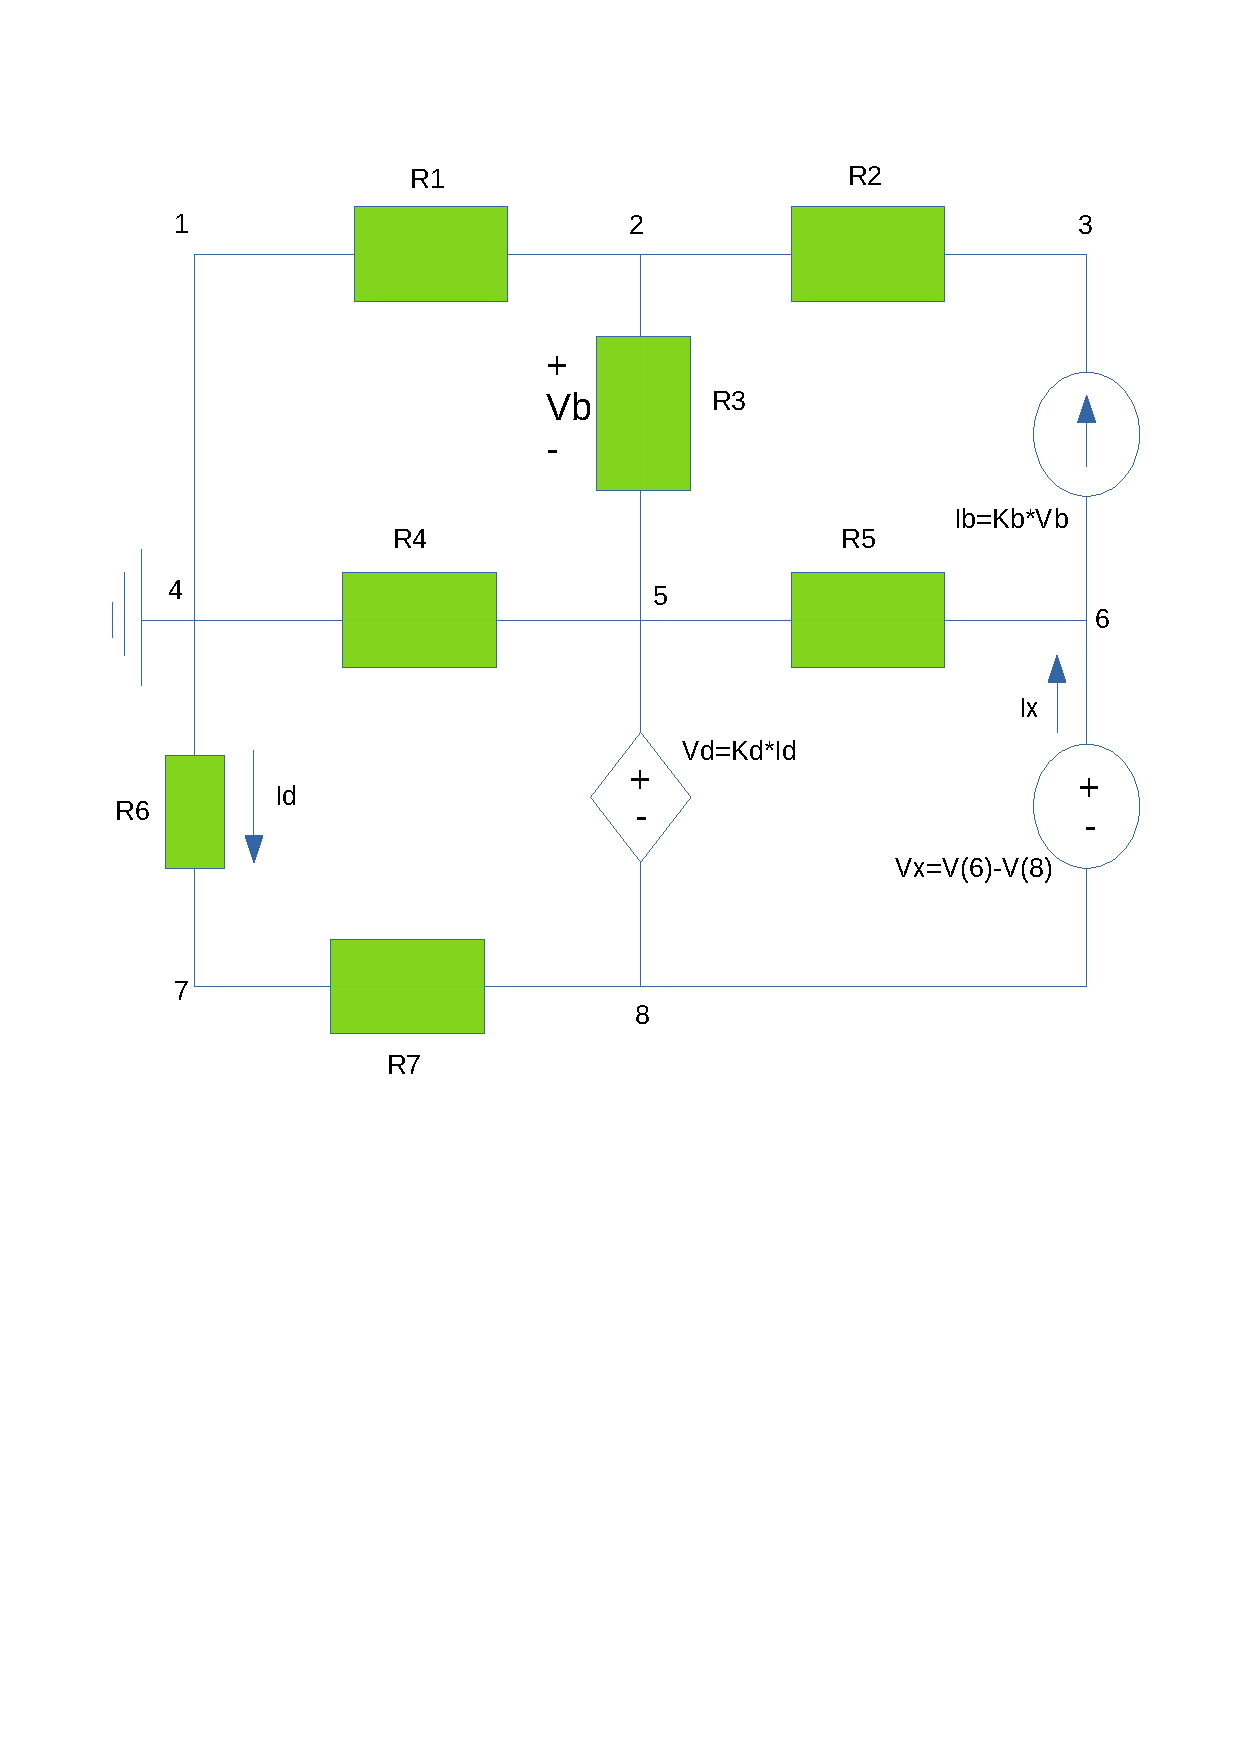
\includegraphics[width=0.6\linewidth]{esquema.pdf}
\caption{Circuit used in 2) to determine $R_{eq}$}
\label{fig:Cir_2)}
\end{figure}

\par Nodal analysis will be done in this circuit where we get the following matrix. Note that in all nodes, we considered divergent currents.

$$
\begin{bmatrix}
0 & 0 & 0 & 1 & 0 & 0 & 0 & 0 \\
-G1 & G1+G2+G3 & -G2 & 0 & -G3 & 0 & 0 & 0 \\
0 & -G2-Kb & G2 & 0 & Kb & 0 & 0 & 0 \\
G1+G4+G6 & -G1 & 0 & 0 & -G4 & 0 & -G6 & 0 \\
1 & 0 & 0 & -1 & 0 & 0 & 0 & 0 \\
0 & 0 & 0 & 0 & 0 & 1 & 0 & 0 \\
0 & 0 & 0 & -G6 & 0 & 0 & G7+G6 & -G7 \\
0 & 0 & 0 & 0 & 0 & 0 & 0 & 1 \\
\end{bmatrix}
\begin{bmatrix}
V_0 \\
V_1 \\
V_2 \\
V_3 \\
V_4 \\
V_5 \\
V_6 \\
V_7  
\end{bmatrix}
=
\begin{bmatrix}
0 \\
0 \\
0 \\
0 \\
0 \\
V(6) \\
0 \\
V(8)  
\end{bmatrix}
$$

\par By solving this matrix we get all node voltages and then by analysing node 6 doing KCL,

\begin{equation}
  I_{x} = Kb(V_2-V_5) - G5(V_5-V_6)
  \label{eq:2)aux1}
\end{equation}

we get $I_x$, and now we can easily get $R_eq$ using Ohm's law,

\begin{equation}
  R_{eq} = \frac{V_x}{I_x}
  \label{eq:2)aux2}
\end{equation}

\par There's still another part of the question, finding the time constant. Since we now have a simple RC circuit the time constant $\tau$ will be $\tau = R_{eq}C$.
\par The following tables shows all the computed results.

\vspace{5mm}
\begin{table}[H]
\centering
\begin{tabularx}{0.6\textwidth} {
  | >{\raggedright\arraybackslash}X
  | >{\raggedleft\arraybackslash}X | }
 \hline
V1 & 0.000000e+00 V \\ \hline
V2 & 8.184440e-01 V \\ \hline
V3 & 2.549645e+00 V \\ \hline
V4 & 0.000000e+00 V \\ \hline
V5 & 7.013583e-01 V \\ \hline
V6 & 5.852787e+00 V \\ \hline
V7 & -2.069080e+00 V \\ \hline
V8 & -3.074760e+00 V \\ \hline

\end{tabularx}
\end{table}

\vspace{5mm}
\begin{table}[H]
\centering
\begin{tabularx}{0.6\textwidth} {
  | >{\raggedright\arraybackslash}X
  | >{\raggedleft\arraybackslash}X | }
 \hline
Vx & 8.589413e+00 V \\ \hline
Ix & 2.465815e-03 A \\ \hline
Req & 3.483397e+03 Ohm \\ \hline
tau & 3.562140e-03 s \\ \hline

\end{tabularx}
\end{table}
\vspace{5mm}

\subsection{Third Point}
\label{ssec:3T}

\noindent \par For the third point, we want to determine the natural solution of the sistem and for that we'll utilise the formula given by the professor in the theoretical classes instead of resolving the differential equation manualy. The formula is 

\begin{equation}
  v(t) = v(\inf) + [v(0) - v(\inf)]e^{-\frac{t}{\tau}}
  \label{eq:form}
\end{equation}

applying to the natural solution of $v_6$ in our circuit, we must find out all the terms of the equation \ref{eq:form}: $\tau=R_{eq}C$ where $R_{eq}$ is the value determined in the second point, the initial condition $v_{6n}(0)$ is equal to $V_x$ and for $v_{6n}(\inf)$ we must know how a capacitor works, in $t<0$ we have a voltage source $Vs$ turned on so our capacitor is receiving charges and charging, after $t=0$ we turn off the voltage source, since we are studying the natural solution, the capacitor discharges and in $t=\inf$ it discharges completely and since there is only dependent sources the voltage in node 6 becames zero. Knowing that, we can now write our equation for $v_{6n}(t)$

\begin{equation}
  v_{6n}(t) = V_x e^{-\frac{t}{\tau}}
  \label{eq:snat}
\end{equation}

\begin{figure}[h] \centering
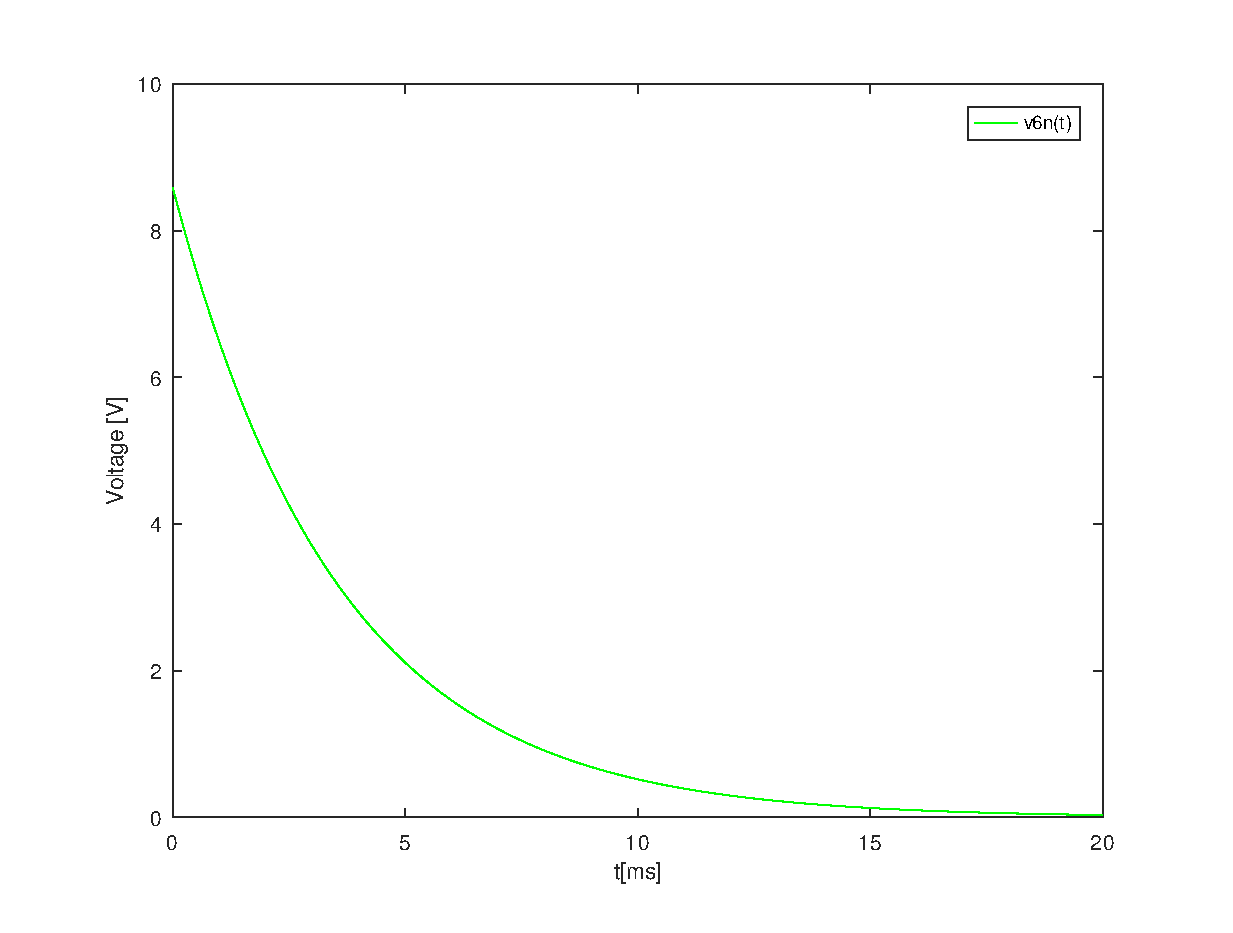
\includegraphics[width=0.7\linewidth]{naturalsolution.eps}
\caption{Natural solution $v_{6n}(t)$, $t\in[0,20]$ms}
\label{fig:snat}
\end{figure}

\subsection{Fourth Point}
\label{ssec:4T}

\par Now in this point we'll analyse the responce of $v_6$ to a sinusoidal signal with a frequency of 1Hz. To do this we use complex notation, because it makes it easier to calculate the amplitude and phase of its response signal. To transfer to the complex notation we simply use 

\begin{equation}
  V\cos(\omega t + \varphi) = \Re (e^{\omega t - \varphi}).
  \label{eq:complex}
\end{equation}

\par Knowing that the frequency response is equal to the impulse frequency and since we now are working with the complex notation shown in \ref{eq:complex} when we do the node analysis in each equation we can divide both terms by $e^{\omega t}$ since it is always greater than zero and in each equation we get what we call "phasors" ($\widetilde{V}=V e^{-\varphi}$) which is the complex amplitude associated to each node that contains the information of the amplitude and phase. Another thing to take in consideration is that since we are now working phasers we will also work with impedance

\begin{equation}
  Z = \frac{\widetilde{V}}{\widetilde{I}}.
  \label{eq:impedance}
\end{equation}

\par In a resistor the impedance is $Z_R=R$, and with a capacitor the impedance is $Z_C=\frac{1}{i\omega C}$, and knowing that we can now do the node analysis to the circuit and determine a matrix that contains all equations from this analysis and determine all node phasors. The matrix is the following,

$$
\begin{bmatrix}
1 & 0 & 0 & 0 & 0 & 0 & 0 & 0 \\
-G1 & G1+G2+G3 & -G2 & 0 & -G3 & 0 & 0 & 0 \\
0 & -G2-Kb & G2 & 0 & Kb & 0 & 0 & 0 \\
0 & 0 & 0 & 1 & 0 & 0 & 0 & 0 \\
0 & 0 & 0 & -KdG6 & -1 & 0 & -KdG6 & 1 \\
0 & Kb & 0 & 0 & -Kb-G5 & G5+i\omega C & 0 & -i\omega C \\
0 & 0 & 0 & -G6 & 0 & 0 & G7+G6 & -G7 \\
0 & -G3 & 0 & -G4 & G3+G4+G5 & -G5-i\omega C & -G7 & G7+i\omega C \\
\end{bmatrix}
\begin{bmatrix}
\widetilde{V_0} \\
\widetilde{V_1} \\
\widetilde{V_2} \\
\widetilde{V_3} \\
\widetilde{V_4} \\
\widetilde{V_5} \\
\widetilde{V_6} \\
\widetilde{V_7}  
\end{bmatrix}
=
\begin{bmatrix}
\widetilde{V_s} \\
0 \\
0 \\
0 \\
0 \\
0 \\
0 \\
0  
\end{bmatrix}
$$

\par Considering $\widetilde{V_s}$ as 1 like it's said we resolve this matrix, and since it has complex numbers in it we'll get also complex numbers for the phasors in all nodes like we want. We can now determine its magnitude and its argument for each phasor, the following table shows exactly that,

\vspace{5mm}

\begin{table}[H]
\centering
\begin{tabularx}{1.0\textwidth} {
  | >{\raggedright\arraybackslash}X
  | >{\centering\arraybackslash}X
  | >{\centering\arraybackslash}X
  | >{\raggedleft\arraybackslash}X | }
 \hline
Amplitude1 & 1.000000e+00 V & Fase1 & 0.000000e+00 graus \\ \hline
Amplitude2 & 9.483936e-01 V & Fase2 & -1.735422e-15 graus \\ \hline
Amplitude3 & 8.415772e-01 V & Fase3 & -3.870526e-14 graus \\ \hline
Amplitude4 & 2.730068e-17 V & Fase4 & 1.800000e+02 graus \\ \hline
Amplitude5 & 9.557102e-01 V & Fase5 & 4.944819e-16 graus \\ \hline
Amplitude6 & 5.638899e-01 V & Fase6 & -1.712249e+02 graus \\ \hline
Amplitude7 & 3.731395e-01 V & Fase7 & -1.800000e+02 graus \\ \hline
Amplitude8 & 5.617171e-01 V & Fase8 & -1.800000e+02 graus \\ \hline

\end{tabularx}
\end{table}

\vspace{5mm}

\subsection{Fifth Point}
\label{ssec:5T}

\par Since we know from \ref{ssec:4T} the response amplitude and phase for all the nodes we can calculate the force solution $v_{6f}(t)$. Calling $A_6$ and $\varphi _6$ to the amplitude and phase of the forced response of node 6, the forced solution will be 

\begin{equation}
  v_{6f}(t) = A_6 \sin(\omega t + \varphi _6)
  \label{eq:fsol}
\end{equation}

where $\omega=2\pi f$ and $f=1Hz$. Now using the superposition theorem we get the final total solution,

\begin{equation}
  v_{6}(t) = v_{6n}(t)+v_{6f}(t) \Rightarrow v_{6}(t) = A_6 \sin(\omega t + \varphi _6) + V_x e^{-\frac{t}{R_{eq}C}}
  \label{eq:gensol}
\end{equation}

where all the values are the ones specified in the previous points. The following plot shows $v_6$ and $vs$ as functions of time.

\begin{figure}[H] \centering
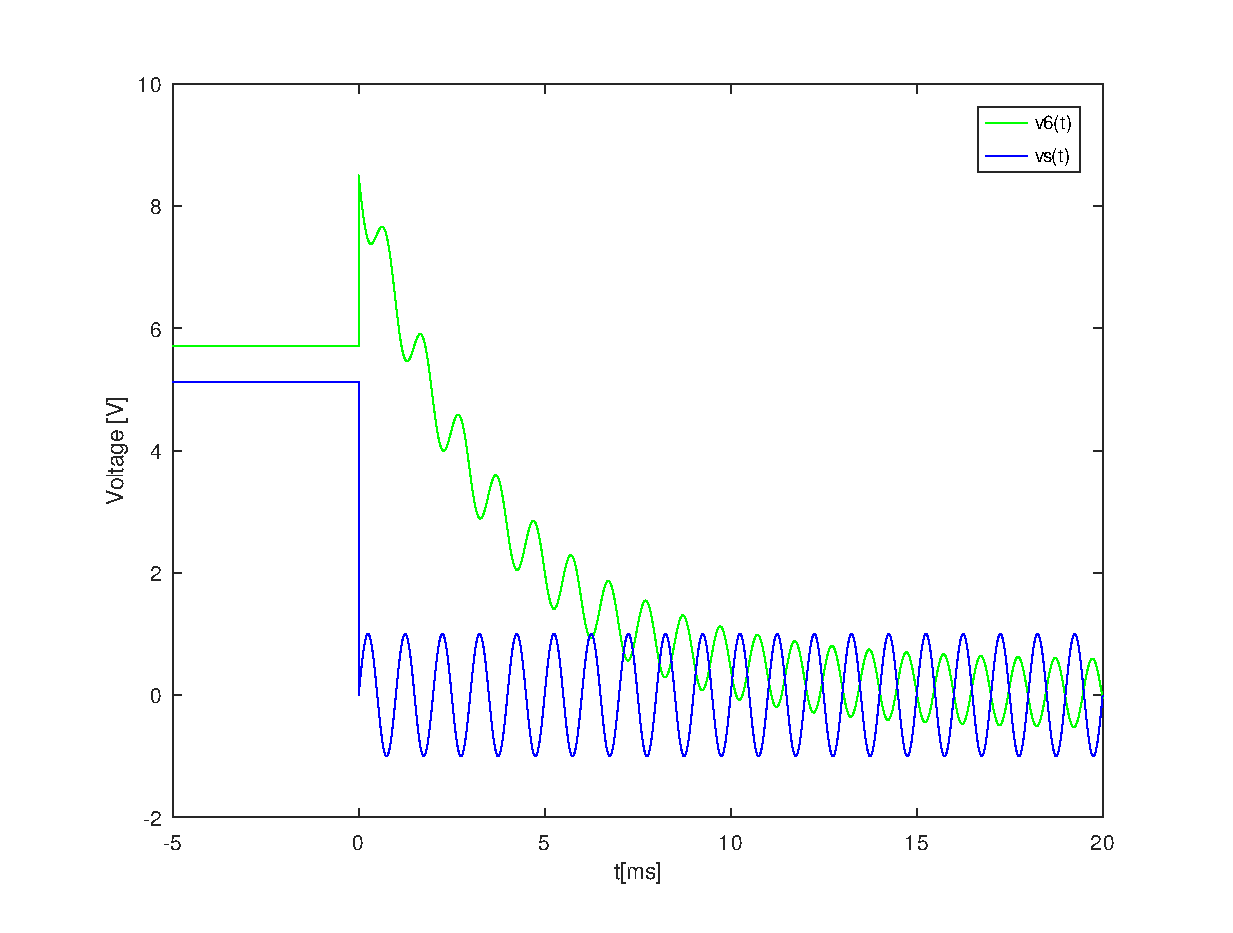
\includegraphics[width=0.7\linewidth]{general_solution.eps}
\caption{Solução total $v_{6}(t)$, $t\in[-5,20]$ ms}
\label{fig:gensol}
\end{figure}

\subsection{Sixth Point}
\label{ssec:6T}

\par In this final point we want to analyse the frequency response of $vs(f)$, $vc(f)$ and in node 6 $(v_6(f))$ for a frequency range 0.1Hz to 1MHz. Note that $vc(f)$ is defined as $v_6(f)-v_8(f)$.
\par To do this we simply apply the same method and matrix used in \ref{ssec:4T} for 200 frequency values logarithmic spaced and then again converting the phasor to amplitude and phase. Another thing o note is that for node 6 we simply use the phaser of node 6, for $vc$ we use the phasor from the previous definition and for $vs$ we use the phaser $v_1 - V_4$. Having done this, we can plot the logarithmic spaced frequency values with the amplitude and phase of each one. The following two graphs shows these functions, 

\begin{figure}[h] \centering
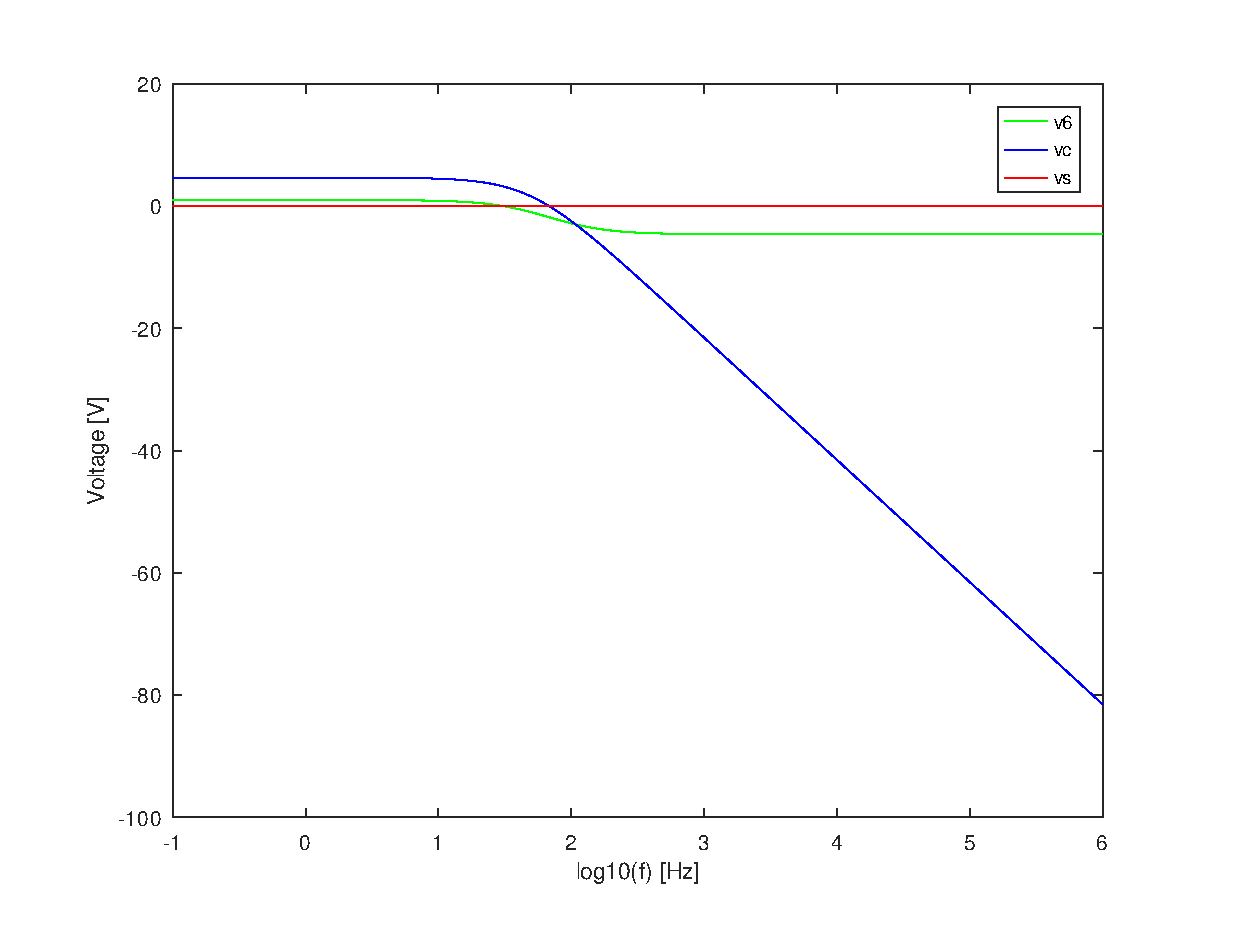
\includegraphics[width=0.7\linewidth]{magnitude(freq).eps}
\caption{Magnitudes as functions of frequency, $f\in[0.1,10^6]$ Hz}
\label{fig:mag(f)}
\end{figure}

\begin{figure}[h] \centering
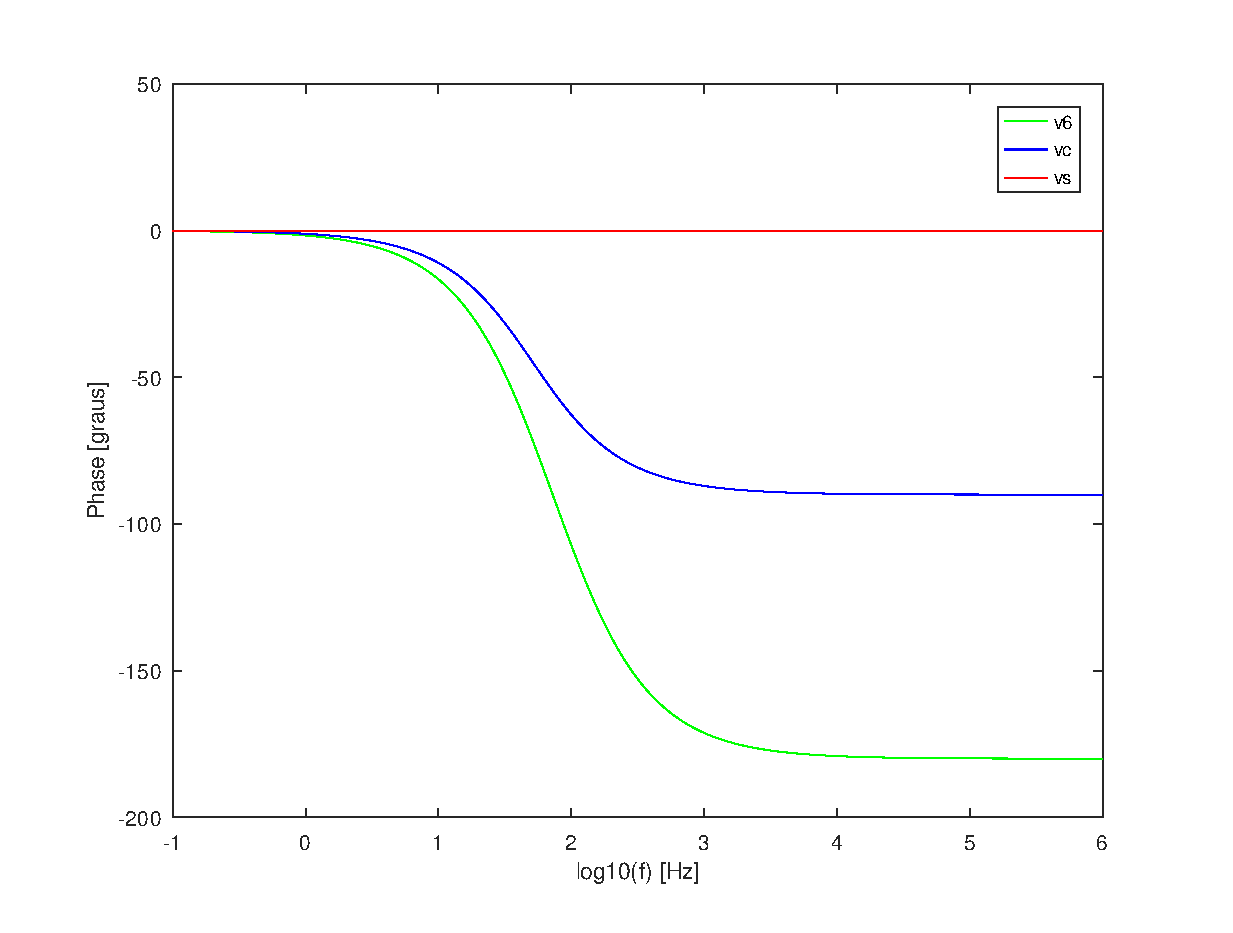
\includegraphics[width=0.6\linewidth]{phase(freq).eps}
\caption{Phases as functions of frequency, $f\in[0.1,10^6]$ Hz}
\label{fig:pha(f)}
\end{figure}

